\documentclass[../main.tex]{subfiles}
\usepackage{silence}
\usepackage{xr}
\NewDocumentCommand{\ExternalDocument}{m}{
	\externaldocument{#1}
	\typeout{No file chapters/#1.aux.}
}
\ExternalDocument{3-SOTA}
\ExternalDocument{2-Background}
\WarningFilter{glossaries}{No \printglossary or \printglossaries found}
\robExtConfigure{disable externalization}
\begin{document}
\ifSubfilesClassLoaded{%
	\graphicspath{{figures/7-Interpretability/}}%
	\setcounter{chapter}{6}%
	\mainmatter%
}{
	\graphicspath{{../figures/7-Interpretability/}}%
}
\chapter{Explaining with counterfactuals}\label{chap:counterfactuals}
\minitocpage
\section{Methods}
	We propose to use \glspl{gan} to generate counterfactual explanations, and the proposed architecture is detailed in \cref{fig:gan_cf}.
	We trained a \gls{wgangp} with extra classifiers, adding more constraints on the generated counterfactual: it does predict the desired class and does not change the tissue of origin.
	The generator can be later used to explain any point with counterfactual.
	To ensure that the generated points are actual counterfactual and not adversarial examples, we trained various models with adversarial training to identify the model with the best accuracy-robustness tradeoff.
	\subsection{\glsfmtshortpl{gan} to generate counterfactuals}
		\begin{figure}[htbp]
			\centering
			\begin{tikzpicture}[inner sep=0pt, very thick]
				\node at (0,0) [square, draw, minimum size=1.5cm] (xin) {\(\symbf{x}\)};
				\node (gen) [right=1cm of xin.east, anchor=west, rounded rectangle, rounded rectangle west arc=none, draw, minimum height=1cm, minimum width=11mm] {\(G\)};
				\node (delta) [right=1.5cm of gen.east, anchor=west,square, draw, minimum size=1.5cm] {\(\delta\)};
				\node (add) [right=5mm of delta.east, anchor=west, draw, circle, minimum size=7.5mm] {};
				\draw (add.north) -- (add.south);
				\draw (add.west) -- (add.east);
				\node (xcf) [right=5mm of add.east, anchor=west,square, draw, minimum size=1.5cm] {\(x^{\text{CF}}\)};
				\node (cl1) [right=1cm of xcf.east, anchor=west, rounded rectangle, rounded rectangle west arc=none, draw, minimum height=1cm, minimum width=11mm] {\(\operatorname{Cl}\)};
				\node (cly) [right=6mm of cl1.east, anchor=west] {\(\hat{y}\)};
				\node (ycf) [right=1.5cm of cly.east, anchor=west] {\(y^{\text{CF}}\)};

				\node (dis) [below=7mm of cl1.south, anchor=north, rounded rectangle, rounded rectangle west arc=none, draw, minimum height=1cm, minimum width=11mm] {\(D\)};
				\node (realfake) at (dis.east -| cly.south)  {\(s\)};
				\node[align=left] (labelrealfake) at (realfake.east -| ycf.south) {0 \\ 1};

				\node (cl2) [above=7mm of cl1.north, anchor=south, rounded rectangle, rounded rectangle west arc=none, draw, minimum height=1cm, minimum width=11mm] {\(\operatorname{Cl}_{T}\)};
				\node (cl2y) at (cl2.east -| cly.north)  {\(\hat{y}_{T}\)};
				\node (ytissue) at (cl2y.east -| ycf.north) {\(y_{T}\)};

				\node (xreal) at (xcf.south |- dis.east) [draw, square, minimum size=1.5cm, double copy shadow={shadow xshift=-.5ex, shadow yshift=.5ex, opacity=.5}, fill=white] {\(\symcal{X}\)};

				\draw[-stealth] (xin.east) -- (gen.west);
				\draw[-stealth] (gen.east) -- node [midway, matrix, draw=none, anchor=center, yshift=0.6em] {
					\node[draw=none,minimum size=1.2em] {\(\symcal{M}\)}; \\
					\node[draw,fill=black,minimum size=1.2em] {};  \\
					\node[draw,fill=white,minimum size=1.2em] {};  \\
					\node[draw,fill=black,minimum size=1.2em] {};  \\
					\node[draw,fill=white,minimum size=1.2em] {};  \\
					\node[draw,fill=black,minimum size=1.2em] {};  \\
					\node[draw,fill=white,minimum size=1.2em] {};  \\
				} (delta.west);
				\draw[-stealth] (delta.east) -- (add.west);
				\draw[-stealth]  (xin.south) -- ++(0,-12mm) -| (add.south);
				\draw[-stealth] (add.east) -- (xcf.west);
				\draw[-stealth] (xcf.east) -- (cl1.west);
				\draw[-stealth] (xcf.east) -- ++(4mm, 0) |- ([yshift=2mm]dis.west);
				\draw[-stealth] ([yshift=-2mm]xreal.east) -- ([yshift=-2mm]dis.west);
				\draw[-stealth] (xcf.east) -- ++(4mm, 0) |- (cl2.west);
				\draw[-stealth] (cl1.east) -- (cly.west);
				\draw[-stealth] (cl2.east) -- (cl2y.west);
				\draw[-stealth] (dis.east) -- (realfake.west);
				\draw[stealth-stealth, dashed] (cly.east) -- node [midway,above, yshift=0.5ex] {\(\symcal{L}_{\operatorname{Cl}}\)}  (ycf.west);
				\draw[stealth-stealth, dashed] (cl2y.east) -- node [midway,above, yshift=0.5ex] {\(\symcal{L}_{\operatorname{Cl}_{T}}\)}  (ytissue.west);
				\draw[stealth-stealth, dashed] (realfake.east) -- node [midway,above, yshift=0.5ex] {\(\symcal{L}_{\text{GAN}}\)}  (labelrealfake.west);
			\end{tikzpicture}
			\caption[Architecture of the counterfactual \glsfmtshort{gan}]{Architecture of the counterfactual \glsfmtshort{gan}. The example \(x\), for which a counterfactual is searched, is passed through the generator \(G\) to obtain the optimal perturbation \(\delta\). This perturbation is added to the input to obtain the counterfactual point \(x^{\text{CF}}\). During the training phase, the counterfactual point is evaluated with two classifiers to ensure the point is classified to the desired class (\(\operatorname{Cl}\)) and belongs to the same tissue as the original point (\(\operatorname{Cl}_{T}\)). A critic \(D\) is used to ensure the generated point belongs to the original data distribution. }\label{fig:gan_cf}
		\end{figure}
		Counterfactual explanations aim to explain a prediction of a sample \(\symbf{x}\) by finding a minimal perturbation \(\delta\) in the data space that will change the prediction.
		The search for a counterfactual explanation can be formulated as an optimization problem (see \cref{eq:opt_cf})~\cite{wachter2017counterfactual}.
		A valid counterfactual is a counterfactual with added properties: \ref{item:cf_actionability}, \ref{item:cf_sparse}, and \ref{item:cf_data_manifold}.
		\Glspl{gan} are a deep learning architecture for generating new samples; it relies on two components a Generator \(G\) capturing the data distribution and a discriminator \(D\) estimating the realness of a sample~(see~\cref{sec:gan})~\cite{Goodfellow2014GAN}.
		As \glspl{gan} are good at capturing data distribution, they can be used to generate counterfactuals respecting the \ref{item:cf_data_manifold} constraint.

		\Cref{fig:gan_cf} presents the overall architecture of the \gls{gan} used for generating counterfactual explanations.
		To obtain a counterfactual, the point \(\symbf{x}\) to explain is passed through the generator \(G\), a \gls{fcn} of \(l\) layers with \gls{relu} intermediate activation and no final activation, to obtain the perturbation \(\delta\).
		To ensure the \ref{item:cf_actionability} property, a binary mask \(\symcal{M}\) is applied element-wise on the generated perturbation to specify which features can be changed.
		\begin{equation}
			\delta = G\left(\symbf{x}\right) \odot \symcal{M}
		\end{equation}
		The counterfactual point or explanation is obtained by adding this perturbation \(\delta\) to the original point: \(\symbf{x}^{\text{CF}} = \symbf{x} + \delta\).

		As \glspl{gan} are known for their training instabilities~\cite{Salimans2016ImprovedTF,Arjovsky2017TowardsPM}, we used a \glsxtrlong{wgangp} (see~\cref{sec:gan})~\cite{WGANGP}.
		The \gls{wgangp} is trained by solving the following optimization problem:
		\begin{multline}
			\min_{G} \max_{D} \symcal{L}_{\text{WGAN}}\left(G,D\right) = \E_{x\sim p_{d}}\left[ D\left(x\right)\right] - \E_{x^{\text{CF}}\sim p_{g}}\left[ D\left(x^{\text{CF}}\right)\right] \\ + \lambda \E_{\tilde{x}\sim p_{g}}\left[ {\left( {\left\|\nabla_{\tilde{x}}D\left(\tilde{x}\right) \right\|}_{2} -1 \right)}^{2}\right] \label{eq:wgan_opt_cf}
		\end{multline}
		where \(p_{d}\) is the true data distribution, \(p_{g}\) is the distribution learned by the generator \(G\), \(\lambda\) is the penalty weight forcing the discriminator \(D\) to be a K-Lipschitz function, and \(\tilde{x}\) is a linearly interpolated point between \(x\) and \(x^{\text{CF}}\).
		The main desiderata of a counterfactual is to change the predicted class of \(\symbf{x}\) from \(\hat{y}\) to \(y^{\text{CF}}\).
		The fullfilment of this constraint is achieved by adding a term \(\symcal{L}_{\operatorname{Cl}}\left(G,\operatorname{Cl}, y^{\text{CF}} \right) = \symcal{L}_{\text{CE}}\left(\operatorname{Cl}\left(x^{\text{CF}}\right),y^{\text{CF}}\right) \) to the optimization problem~(\cref{eq:wgan_opt_cf}), where \(\operatorname{Cl}\) is a pretrained classifier and \(\symcal{L}_{\text{CE}}\) the cross-entropy loss~(see~\cref{eq:ce_loss}).
		The \ref{item:cf_sparse} constraint of a counterfactual is obtained by adding a \(L_{1}\) regularization on the generated perturbation \(\delta\) to the optimization problem~(\cref{eq:wgan_opt_cf}): \(\symcal{L}_{\text{Reg}}\left(G\right) = \left\|G\left(x\right) \odot \symcal{M}\right\|_{1}\).
		More constraints can be added to the generator by adding other loss terms to the optimization problem.
		For instance, in our scenario we added a loss term \(\symcal{L}_{\operatorname{Cl}_{T}}\left(G,\operatorname{Cl}_{T}, y_{T} \right) = \symcal{L}_{\text{CE}}\left(\operatorname{Cl}_{T}\left(x^{\text{CF}}\right),y_{T}\right)\) to ensure that the generated counterfactual belongs to the correct tissue type, where \(\operatorname{Cl}_{T}\) is a pretrained tissue classifier.
		Finally, the counterfactual \gls{gan} is trained by solving the following optimization problem:
		\begin{multline}
			\min_{G} \max_{D} \symcal{L}_{\text{WGAN}}\left(G,D\right) + \symcal{L}_{\operatorname{Cl}}\left(G,\operatorname{Cl}, y^{\text{CF}}\right)\\ + \symcal{L}_{\operatorname{Cl}_{T}}\left(G,\operatorname{Cl}_{T}, y_{T}\right) + \symcal{L}_{\text{Reg}}\left(G\right)
		\end{multline}

	\subsection{Counterfactuals evaluation}
		To evaluate the generated counterfactual examples, we used metrics to evaluate the different counterfactual properties.
		The effectiveness of our approach, \ie{}the capacity of the method to generate counterfactuals that do change the prediction, was measured using counterfactual accuracy: \(\symcal{A}_{\text{CF}}\).
		The counterfactual accuracy compares the prediction obtained by the classifier \(\operatorname{Cl}\) from the counterfactual \(\symbf{x}^{\text{CF}}\) to the desired class \(y^{\text{CF}}\).
		The closeness of the counterfactual to the original point was determined using various measure distances based on \(L_{1}\), \(L_{2}\), or \(L_{\infty}\) norms.
		The sparsity of the perturbation was evaluated with the \(L_{0}\)-\textit{norm}\footnote{Here, norm is in italics as this is not a proper norm. The \(L_{0}\)-\textit{norm} is not homogeneous: \(\left\|\lambda x \right\|_{0} \neq \left|\lambda\right| \left\| x \right\|_{0}\)}, measuring the number of nonzeros elements in a vector, defined as\footnote{This \textit{norm} can also be seen as the hamming distance of a vector \(x\) with the zero vector \(\symbb{0}_{n}\): \(\sum_{i=1}^{n} \symbb{1}\left(x \neq \symbb{0}_{n}\right)_{i}\)}: \(\sum_{i=1}^{n} \left|x_{i}\right|^{0}\) with defining that \(\left|0\right|^{0}=0\).
		The realism of counterfactuals was evaluated by measuring how much training data supports the generated counterfactual, \ie{} justify the counterfactual by connecting it to real data~\cite{JustifyCF}.
		A realistic counterfactual should have points in its neighborhood that have the same label \( y^{\text{kNN}}\) as the desired class \(y^{\text{CF}}\), this can be computed as the proportion of point in the k-neighbors agreeing with the counterfactual class: \(\symcal{A}_{\text{kNN}} = \frac{1}{k}\sum_{i=1}^{k}\symbb{1}\left(y^{\text{CF}},  y^{\text{kNN}}_{i}\right)\)~\cite{Carla_CF}.
		This metric is only considered for correct or effective counterfactual, generated point \(\symbf{x}^{\text{CF}}\) that are predicted as \(y^{\text{CF}}\).
		Another way of checking the realism of counterfactuals is by visualizing the position of the counterfactual projected into the UMAP space generated from training data.

		For real case scenarios, an important characteristic is the time required to get a counterfactual from an example.
		This characteristic is evaluated by measuring the latency, the time to get a prediction for a single example.

	\subsection{Getting a robust model: adversarial training}
		Adversarial examples are inputs specifically designed to fool a neural network but are crafted to be \textit{indistinguishable}\footnote{This term originates from the development of adversarial examples in the computer field where the meaning of \textit{indistinguishable} is clear. For other application fields, the meaning needs to be adapted.
			Usually, a notion of minimal distance is introduced.} from a real input~(\cref{box:adversarial})~\cite{Szegedy2013IntriguingPO}.
		Those examples are generated with adversarial attacks such as \gls{pgd}~\cite{PGDAttacks2} or Carlini and Wagner attack~\cite{Carlini2016TowardsET}.
		As those attacks solve similar optimization problems as counterfactuals generation methods~\cite{Pawelczyk2021ExploringCE,Freiesleben2021}, it is important to prevent the \gls{gan} from generating adversarial examples instead of counterfactuals.
		In the proposed architecture, the classifier \(\operatorname{Cl}\) is the component sensitive to adversarial examples as it is used to classify the generated points.
		The classifier can be made robust to adversarial examples with untargeted adversarial training~\cite{AdvTrainingMinMax}, which is achieved by solving the following min-max optimization problem:
		\begin{equation}
			\min_{\operatorname{Cl}} \E_{(x,y)}\left[\max_{\delta^{\star} \in \Delta} \symcal{L}_{\text{CE}}\left(\operatorname{Cl}\left(x+\delta^{\star}\right), y \right)  \right]
		\end{equation}
		where \(\symcal{L}_{\text{CE}}\) is the cross-entropy loss, \(\delta^{\star}\) the minimal adversarial perturbation changing the prediction and \(\Delta\) is the allowed set of perturbation.
		The algorithm used to have a robust classifier \(\operatorname{Cl}\) is presented in \cref{alg:adv_training}.
		\begin{algorithm}[htbp]
			\DontPrintSemicolon
			\KwIn{\(\operatorname{Cl}\), its parameters \(\theta_{\operatorname{Cl}}\) and \(\epsilon\) the size of the attack}
			\KwOut{Robust classifier \(\operatorname{Cl}\)}
			\For{\(T\) training steps}{
			\For{\(B\) mini-batches}{
			Sample a batch \(x,y\) from the training data\;
			Perfrom an adversarial attack:\;
			\(\delta^{\star} = \operatorname{AdvAttack}\left(x,y,\epsilon\right)\)\;
			Update classifier weights:\;
			\( \theta_{\operatorname{Cl}} \leftarrow \theta_{\operatorname{Cl}} - \eta \nabla_{\theta_{\operatorname{Cl}}}\symcal{L}_{\text{CE}}\left(\operatorname{Cl}\left(x+\delta^{\star}\right), y\right) \)\;
			}
			}
			\caption{Adversarial training of the classifier \(\operatorname{Cl}\)}\label{alg:adv_training}
		\end{algorithm}
		As adversarial attacks can be targeted, a variant of adversarial training can be used where adversarial examples are generated by randomly targeted attacks.
		This strategy can increase the robustness as the attacks are made in multiple directions.


	\subsection{Adversarial Metrics}
		To evaluate the robustness of the classifier \(\operatorname{Cl}\), we used three metrics: model smoothness~\cite{MarginDecision}, margin decision~\cite{MarginDecision} and boundary thickness~\cite{AdvBoundaryThick}.
		The details of each metric are given below:
		\begin{description}[
				style=multiline,
				leftmargin=!,
				labelwidth=2.5cm
			]
			\item[Model smoothness]
				This metric measures the insensitiveness of the output to the input perturbation~\cite{MarginDecision}, \ie{} the decision boundary is further away from samples, and small perturbation does not affect the output.
				This metric is defined as the Kullback-Leibler divergence between the predicted probability of a clean sample \(\operatorname{Cl}\left(\symbf{x}\right)\) and the predicted probability of the corresponding adversarial example \(\operatorname{Cl}\left(\symbf{x}^{\star}\right)\):
				\begin{equation}
					\operatorname{KL}\left(\operatorname{Cl}\left(\symbf{x}\right) \| \operatorname{Cl}\left(\symbf{x}^{\star}\right)\right)
				\end{equation}
				A smaller smoothness indicates a more robust model.
			\item[Margin decision]
				This metric measures the distance of an example to the decision boundary~\cite{MarginDecision}.
				This is measured as the difference between the probability of the true label \(\operatorname{Cl}\left(\symbf{x}\right)_{y}\) and the probability of the other most probable class \(\max_{i \neq y} \operatorname{Cl}\left(\symbf{x}\right)_{i}\):
				\begin{equation}
					\operatorname{Cl}\left(\symbf{x}\right)_{y} - \max_{i \neq y} \operatorname{Cl}\left(\symbf{x}\right)_{i}
				\end{equation}
				A higher margin decision is better.
			\item[Boundary thickness]
				The boundaries thickness measures the margin of the region where the probability difference \(D_{ij}\left(\cdot\right) = \operatorname{Cl}\left(\cdot\right)_{i} - \operatorname{Cl}\left(\cdot\right)_{j}\), where \(i\) and \(j\) are the predicted labels of a clean sample \(\symbf{x}\) and its adversarial example \(\symbf{x}^{\star}\), lies between two values \(\alpha\) and \(\beta\)~\cite{AdvBoundaryThick}:
				\begin{equation}
					\left\|x - x^{\star}\right\|_{2} \int_{0}^{1} \symbb{1}\left\{ \alpha < D_{ij}\left(tx + \left(1-t\right)x^{\star} \right) < \beta\right\}
				\end{equation}
				Thicker boundary helps improve robustness against adversarial examples.
		\end{description}


\section{Preliminary results}
	\subsection{Adversarial study}
		Batch normalization was rapidly identified as problematic for learning robust models with adversarial training~\cite{AdvBNProblems,xie2019intriguingpropertiesadversarialtraining}.
		Indeed, batch normalization was designed to learn statistics from a single distribution: introducing adversarial examples in a batch creates batches with data from two distributions.
		This leads to incorrect statistics estimates, which hinders performances~\cite{AdvBNProblems,BNAdvStats}.
		To palliate those problems, \citeauthor{AdvBNProblems} use two parallel batch normalizations: one only receives clean examples to correctly estimate clean statistics while the other only receives adversarial examples~\cite{AdvBNProblems}.
		However, there is no oracle to route an example to the correct batch normalization.
		More recent work studied adversarial training on models without any normalization layers~\cite{wang2022removing}, to prevent covariate shift\footnote{Batch normalization was initially proposed to mitigate this internal covariate shift, the change of layer activation distributions due to the evolution of the parameters during training.} from occurring in the hidden layers, weights of layer \(l\) are standardized~\cite{brock2021characterizing}:
		\begin{equation}
			\hat{W}^{l}_{ij} = \gamma\frac{W^{l}_{ij} - \mu^{l}_{i}}{\sigma^{l}_{i}\sqrt{F^{l}_{\text{in}}}}
		\end{equation}
		where \(\gamma\) is a scaling factor depending on the type of non-linearities~\cite{brock2021characterizing}, \(\mu^{l}_{i}\) and \(\sigma^{l}_{i}\) are the mean and standard deviation of  the \(i\)-th row of \(W^{l}\) and \(F^{l}_{\text{in}}\) is the number of input elements of the layer, \ie{}the batch size for linear layers.

		To identify the most robust classifier \(\operatorname{Cl}\), we compared the tradeoff accuracy robustness of five models: an \gls{mlp} with batch normalization (\glsxtrshort{mlp} BN), an \gls{mlp} with layer normalization (\glsxtrshort{mlp} LN), an \gls{mlp} without any normalization layer (\glsxtrshort{mlp} NoNorm), a norm-free \gls{mlp} where weights are standardized (\glsxtrshort{mlp} NF) and an \glsxtrshort{mlp} NF where \gls{agc} is used during training (\glsxtrshort{mlp} NF \glsxtrshort{agc}).
		\Gls{agc} was introduced in~\cite{NoNormApplied} to improve training stability on larger batches by controlling the magnitude of the gradients according to the ratio of gradient norms to parameter norms and ensuring balanced updates.
		Adversarial training benefits from \textit{showing} adversarial examples to the models, and there are various ways of finding adversarial examples~(\cref{box:adversarial}).
		We selected a 10-step \gls{pgd} attack with an \(L_{\infty}\)-norm implemented with the {\sourcecode rai-toolbox}~\cite{soklaski2022toolspracticesresponsibleai}.
		An important parameter of \gls{pgd} attacks is the set allowed perturbation \(\Delta\) defined by \(\epsilon\).
		The maximum allowed \(\epsilon\) value was set to the minimal \(L_{\infty}\) distance between points of two different classes\footnote{choosing a higher epsilon will guarantee the existence of an adversarial example, \ie{} a point of another class.}~(\cref{fig:dist_cls_distibutionLinf}).
		Adversarial training introduces an implicit task: the model robustness, which changes the training dynamics as the adversarial distributions evolve during training.
		We noticed that with a very large number of training steps\footnote{four times more than \gls{mlp} NF.} the \gls{mlp} BN was able to benefit from adversarial training.
		After identifying the optimal number of training steps for each model, we compared the robustness accuracy tradeoff of the models to \gls{pgd} attacks of various sizes~(\cref{fig:mlp_bn_adv_tradeoff,fig:mlp_ln_adv_tradeoff,fig:mlp_nonorm_adv_tradeoff,fig:mlp_fn_adv_tradeoff,fig:mlp_fnagcadv_tradeoff}) after a clean training (\(\epsilon = 0\)) or an adversarial training (\(\epsilon > 0\)).
		Results for the \gls{mlp} BN model are describe here~(\cref{fig:mlp_bn_adv_tradeoff}), results for the other models  are available in~\cref{chap:interpretability_appendix} \crefrange{fig:mlp_ln_adv_tradeoff}{fig:mlp_fnagcadv_tradeoff}.
		We noticed that adversarial training with a fixed \(\epsilon\) leads to robustness to attacks of the same size.
		Intuitively, adversarial training with large \(\epsilon\) would provide robustness to attacks with smaller \(\epsilon\).
		From our experiments, we observed that was not the case.
		For instance, after adversarial training with \(\epsilon = 0.3\), the highest measured robustness was when attacking with \(\epsilon=0.3\) and there is very limited robustness to smaller attacks.
		Such observation comes from the high dimensionality of omics data.
		Indeed, in high dimension, most of the volume of an \(\epsilon\)-ball\footnote{The set of points at a distance at most \(\epsilon\) from the ball center. The ball can be centered anywhere in the space.} is concentrated near its surface, in other words most of the considered points during the adversarial attack are at a distance \(\epsilon\) of the point being attacked.
		The highest robustness is achieved when training with \(\epsilon=0.1\) attacks, and other sizes of attacks lead to smaller robustness.

		\begin{figure}[htbp]
			\centering
			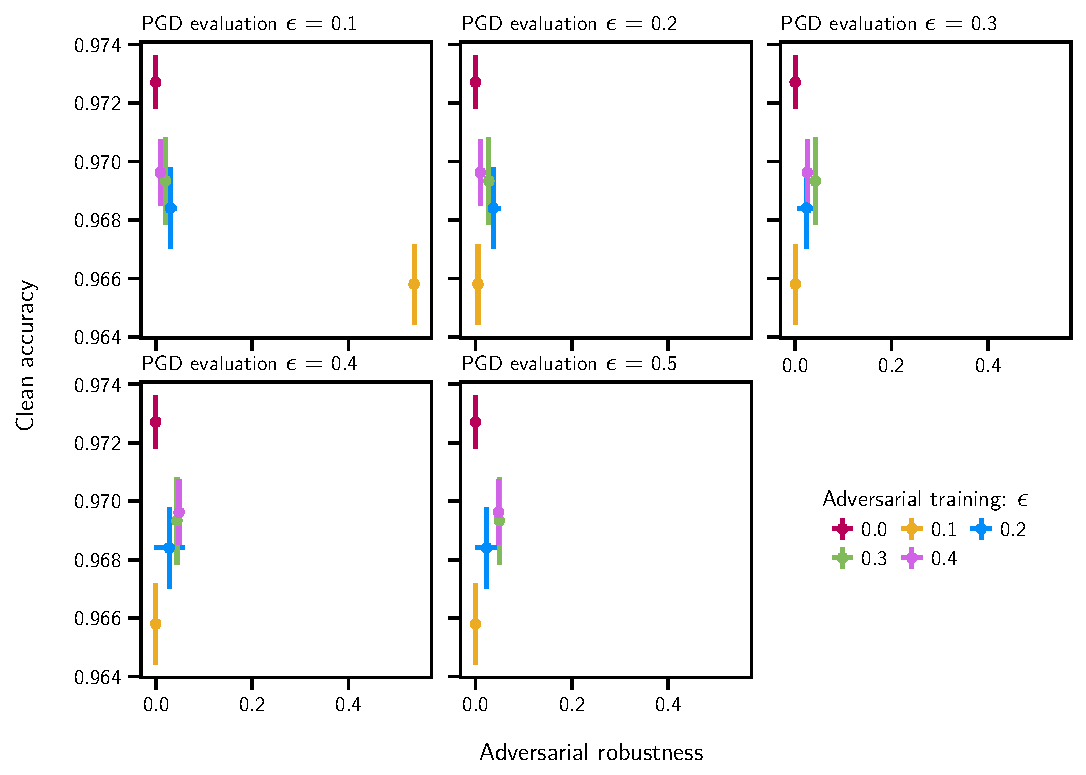
\includegraphics[scale=0.9]{MLP_BN_adversarial_tradeoff.pdf}
			\caption[\glsfmtshort{mlp} BN adversarial robustness-accuracy tradeoff]{Comparison of the adversarial robustness-accuracy tradeoff for \glsfmtshort{pgd} attacks with different sizes (\(\epsilon > 0\)) after adversarial training of the \glsfmtshort{mlp} BN model with various \glsfmtshort{pgd} attacks sizes, \(\epsilon = 0\) corresponds to a classical training on only clean samples.}\label{fig:mlp_bn_adv_tradeoff}
		\end{figure}

		In the following, \(\epsilon = 0.1\) will be used for \gls{pgd} attacks.
		\Cref{fig:adv_robust_strat} compares the robustness-accuracy tradeoff with different training strategies: clean training, untargeted, and targeted adversarial training.
		For all considered models, both targeted and untargeted adversarial training improve robustness while sacrificing some clean accuracy~(\crefrange{fig:adv_robust_strat_mlp_bn}{fig:adv_robust_strat_mlp_fn_agc}).
		For all considered models, the untargeted adversarial training leads to the best robustness compared to the targeted strategy~(\cref{fig:adv_robust_strat}), approximately two times higher robustness.
		The highest robustness ease achieved with untargeted adversarial training for \gls{mlp} BN, \gls{mlp} NF and \gls{mlp} NF AGC~(\cref{fig:adv_robust_strat_mlp_bn,fig:adv_robust_strat_mlp_fn,fig:adv_robust_strat_mlp_fn_agc}).
		For two models, \gls{mlp} NF and \gls{mlp} NF AGC, the loss of accuracy is higher than the other models while achieving better robustness than for the other three~(\cref{fig:adv_robust_strat_mlp_fn,fig:adv_robust_strat_mlp_fn_agc}).
		Going from zero robustness to \(0.5\) robustness is a major improvement.
		Other adversarial training strategies need to be explored to see if the robustness can be increased~\cite{AdvTrainSurvey}.

		\begin{figure}[htbp]
			\centering
			\begin{subcaptiongroup}
				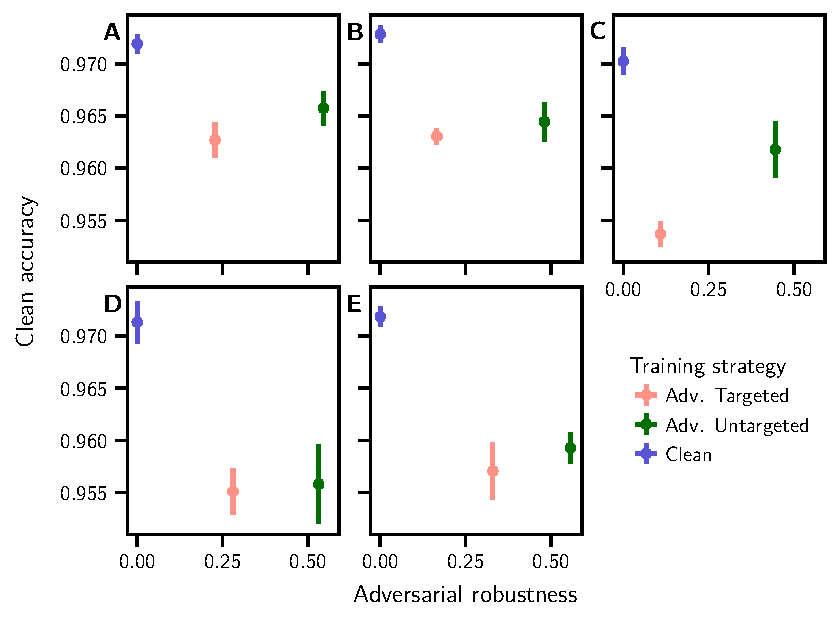
\includegraphics{adversarial_robustness_strategy.pdf}
				\phantomcaption\label{fig:adv_robust_strat_mlp_bn}
				\phantomcaption\label{fig:adv_robust_strat_mlp_ln}
				\phantomcaption\label{fig:adv_robust_strat_mlp_nonorm}
				\phantomcaption\label{fig:adv_robust_strat_mlp_fn}
				\phantomcaption\label{fig:adv_robust_strat_mlp_fn_agc}
			\end{subcaptiongroup}
			\caption[Comparison of the accuracy-robustness tradeoff with various training strategies]{Comparison of the accuracy-robustness tradeoff between three training strategies: clean training, untargeted adversarial training and targeted adversarial training for five models: \glsfmtshort{mlp} BN~\subref{fig:adv_robust_strat_mlp_bn}, \glsfmtshort{mlp} LN~\subref{fig:adv_robust_strat_mlp_ln}, \glsfmtshort{mlp} NoNorm~\subref{fig:adv_robust_strat_mlp_nonorm}, \glsfmtshort{mlp} NF~\subref{fig:adv_robust_strat_mlp_fn}, and \glsfmtshort{mlp} NF \glsfmtshort{agc}~\subref{fig:adv_robust_strat_mlp_fn_agc}.}\label{fig:adv_robust_strat}
		\end{figure}

		In the following, an untargeted adversarial training strategy will be used to increase the model's robustness.
		\Cref{tab:metrics_adv} presents a comparison of boundary thickness, margin decision, and model smoothness of the five considered models after clean training (Robust \xmark) and adversarial training (Robust \cmark).
		The metrics were measured on all samples from the validation set, and their mean value was reported.
		For all considered models, adversarial training leads to thicker boundaries, and the increase is more noticeable for the \gls{mlp} NF and \gls{mlp} NF AGC models.
		Small reductions of the margin decision were observed, but the margins were already high and almost maximal\footnote{The margin decision belongs to the interval \(\left[-1, 1\right]\)}.
		The model smoothness was significantly improved for all models, and the models are more robust to small perturbations of the inputs after adversarial training.

		\begin{table}[htbp]
			\sisetup{round-mode=places,round-precision=2,detect-mode}
			\centering
			\caption[Adversarial metrics comparison]{Comparison of boundary thickness, margin decision, and model smoothness of adversarially trained (Robust \cmark), or not (Robust \xmark), models with different normalization strategies.}\label{tab:metrics_adv}
			\csvreader[
				no head,
				after table={
						\TextArrow{bt1}{bt2}{5pt}
						\TextArrow{md1}{md2}{5pt}
						\TextArrow{ms2}{ms1}{5pt}
					},
				tabularray={%
						colspec={%
								Q[r,m]
								Q[si={table-format=1.2,table-number-alignment=center},c , wd=1.3cm]%
								Q[si={table-format=1.2,table-number-alignment=center},c , wd=1.3cm]%
								Q[si={table-format=1.2,table-number-alignment=center},c , wd=1.3cm]%
								Q[si={table-format=1.2,table-number-alignment=center},c , wd=1.3cm]%
								Q[si={table-format=2.2,table-number-alignment=center},c , wd=1.5cm]%
								Q[si={table-format=1.2,table-number-alignment=center},c , wd=1.5cm]%
							},%
						row{1-2} = {guard},
						row{2} = {c,m, font=\small},
						row{3-Z} = {font=\footnotesize},
						row{4-Z} = {abovesep=1pt},
						row{3-Y} = {belowsep=1pt},
						row{1} = {font=\small\bfseries},
						cell{1}{2} = {r=1,c=2}{c, wd=2.6cm},
						cell{1}{4} = {r=1,c=2}{c, wd=2.6cm},
						cell{1}{6} = {r=1,c=2}{c, wd=3cm},
						%cell{7}{3} = {font=\bfseries},
						hline{1} = {2-Z}{2pt},%
						hline{Z} = {2pt},%
						hline{2-3} = {1pt},%
						column{even} = {rightsep=1pt},
						column{odd[3-Z]} = {leftsep=1pt},
						%cell{3-Z}{1} = {font=\normalsize}
					}
			]{%
				\ifSubfilesClassLoaded{%
					data/AdversarialMetrics.csv%
				}{%
					../data/AdversarialMetrics.csv%
				}%
			}{}{\csvlinetotablerow}
		\end{table}

		As we proposed to characterize counterfactuals with their nearest neighbors, we look at the neighbors of adversarial examples~(\cref{fig:mlp_bn_knn_comp}).
		Adversarial examples are obtained by adding a small perturbation to an original point that will change the prediction.
		The perturbation is considered minimal, and the resulting adversarial is expected to be close to the original point and, therefore, have similar neighbors.
		For the non-robust model, the label obtained from the neighbors \(Y^{\text{kNN}}\) is consistent with model predictions \(\hat{Y}\)~(\cref{fig:mlp_bn_knn_comp}).
		As expected from the previous experiments, the model is not robust, and we were able to find adversarial examples for each sample.
		In the adversarial labels \(\hat{Y}_{adv}\), not all classes are represented, and the normal class is overrepresented.
		The neighborhood of the adversarial samples is similar to the neighborhood of clean samples, and labels obtained from the neighbors \(Y^{\text{kNN}}_{adv}\) are similar to the \gls{knn} label from the clean samples.
		Similar observations are made for targeted attacks.
		For all points, a perturbation was found to change the prediction to the normal class, and the neighborhood predictions correspond to the clean prediction.
		Adversarial training did increase the model's robustness, as an adversarial example is not found for all samples.
		Some classes (PRAD, THCA, LGG) were particularly robust to adversarial attacks.
		For samples where we did find an adversarial, the neighborhood was not similar to the original neighborhood.
		It is also more challenging to find a targeted adversarial example even though we did not explicitly train the model to be robust to this attack.

		\begin{figure}[htbp]
			\centering
			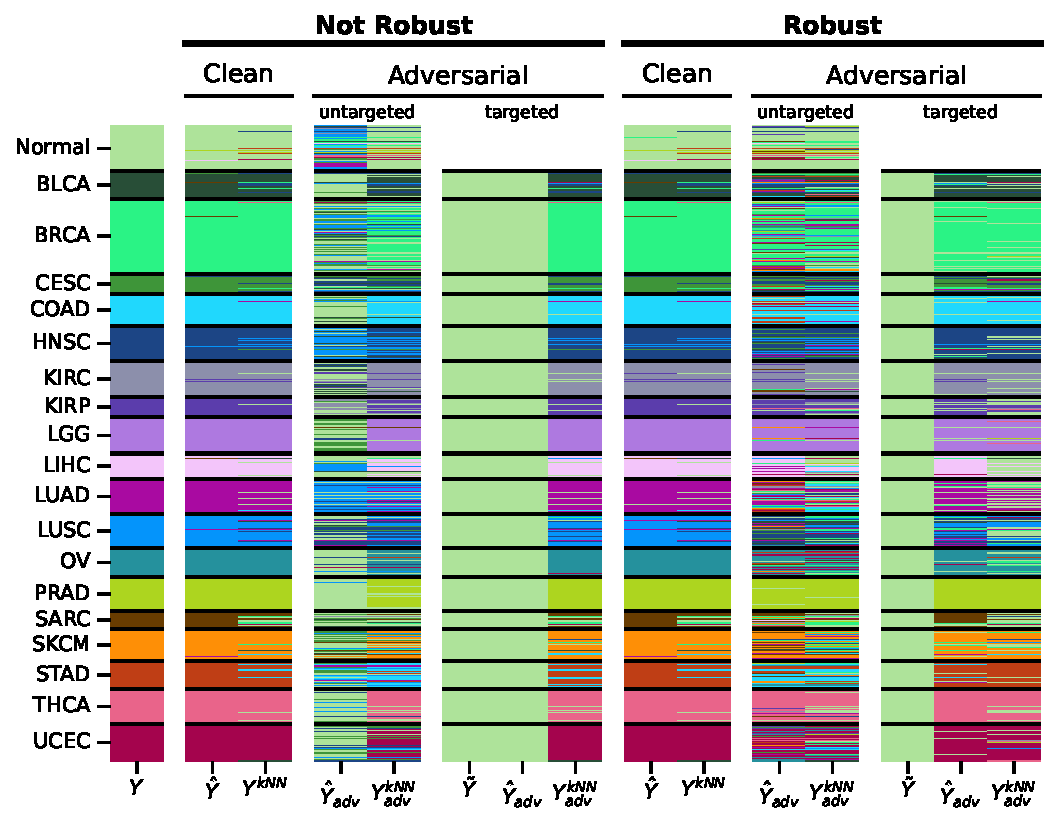
\includegraphics[width=\textwidth]{MLP_BN_knn_comparison.pdf}
			\caption[\glsfmtshort{knn} characterization of adversarial examples with \glsfmtshort{mlp} BN]{\glsfmtshort{knn} characterization of adversarial examples with \glsfmtshort{mlp} BN after clean training (Not Robust) and adversarial training (Robust). For both training strategies we compared untargeted and targeted attacks. \(Y\) represents the true label, \(\hat{Y}\) the predicted class by the model, \(Y^{\text{kNN}}\) the majority voting from the 20 nearest neighbors, \(\hat{Y}_{adv}\) the predicted class of the found adversarial example, \(Y^{\text{kNN}}_{adv}\) the majority voting from the 20 nearest neighbors of the found adversarial, and \(\tilde{Y}\) the desired class of targeted attackes. We set \(\tilde{Y}\) to normal for all samples.}\label{fig:mlp_bn_knn_comp}
		\end{figure}

	\subsection{Counterfactuals}
		% counterfactuals, could we compare the proposed treatments with, when available, the treatment scheme of the patient.

\end{document}
